\chapter[Multiplanar Imaging]{Autonomous Imaging of Multiplanar Regions through
Quadcopter}
\label{ch:multiplanar}
\section{Introduction}
Consider a visit to the art gallery or a tour to ancient temples for restoration. In
such scenarios, we would like to get an unrolled view of scenes depicted on
the walls. We need to capture each surface orthographically from close range to
get minute details required for further work. We may use SLR cameras or even
smartphones having high-resolution cameras which are easily available for
imaging such scenes. Many of these cameras also have special modes to capture
panoramas.
\begin{figure}[h!]
\centering
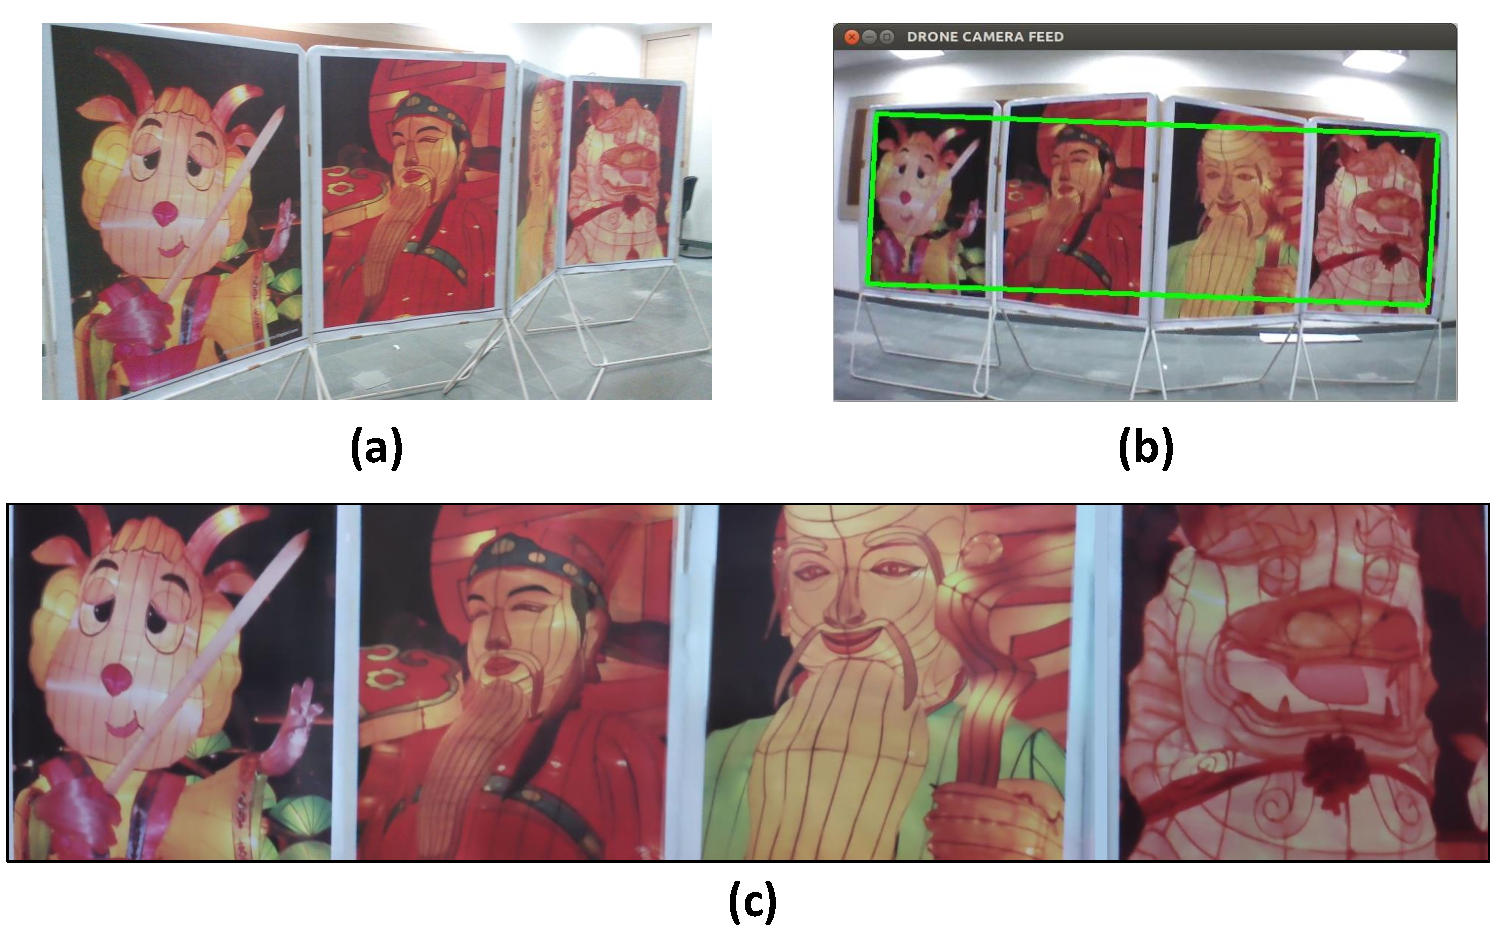
\includegraphics[width=0.98\linewidth]{figures/multiplanar/teaser2}
\caption[Overview of multiplanar imaging]{The multiplanar scene to be mosaiced
is shown in (a).
Long range photograph doesn't give details of all images. The quadcopter has to be moved back
to allow the user to select the area of interest as shown in (b).
Final mosaicing output from this paper is shown in (c). Size of our output is
3427 x 863 pixels.}
\label{fig:teaser}
\end{figure} 

\begin{figure}[htb]
\centering
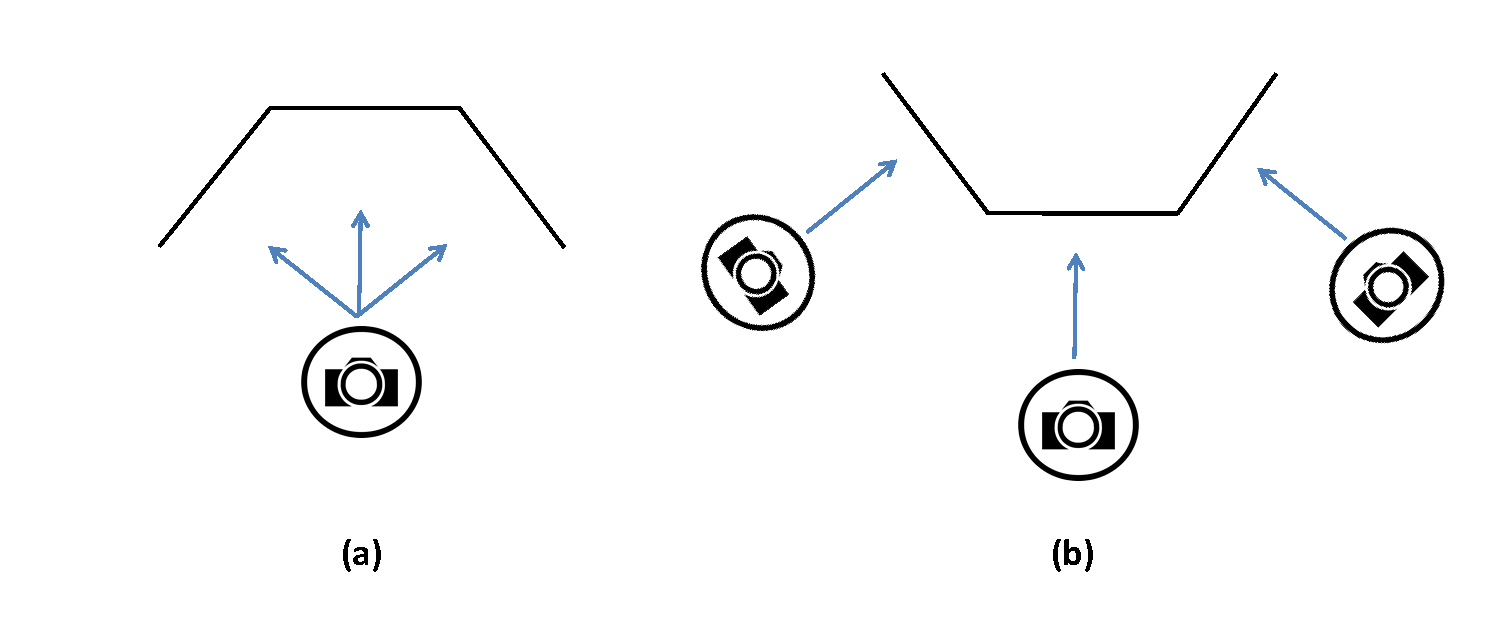
\includegraphics[width=\textwidth]{figures/multiplanar/ConcaveConvex}
\caption[Imaging concave surfaces versus convex surfaces ]{(a) Imaging concave
surfaces. We do not have to change our position, changing orientation is
sufficient to capture the whole surface. (b) While imaging convex surface, one
need to change the position as well as the viewing angle. It makes the process
of building homography based panorama  theoretically impossible.}
\label{fig:convex_concave}
\end{figure}

But practically, when we use such cameras for capturing panoramas, we do not
get the close-up orthographic view of the scenes present at height or not
easily accessible. We also need a steady hand for a long time while capturing
panoramas which might be too tiring.

The limitation of even an expensive SLR cameras is that it can create a panorama with
an orthographic view, only if the surface to be imaged is present on a single
plane. If the surface is concave and the camera is kept at the center of the
surface, only then we get panorama with an orthographic view (Figure
\ref{fig:convex_concave}(a)). But if the surface (or part of it) is convex (Figure \ref{fig:convex_concave}(b),
 viewpoint (along with the orientation) needs to be changed while imaging which
 prohibits the use of panorama mode of most cameras. Even if any camera allows such panorama creation, the output
is distorted due to change in homography. 

In scenarios where handheld devices cannot capture orthographic view of the
input scene, or if the scene is too large, an inexpensive flying device such as
a quadcopter can be used. A quadcopter can cover any large scene with
an orthographic view with precise details (e.g., facial features of a person in
Figure \ref{fig:teaser}) by flying in front of each part of the scene.
Even if we use a quadcopter, manually controlling the quadcopter to image a
large scene spread over multiple planes is a tedious task and hence require
automation.

\textbf{Problem Definition}
In \cite{Prasad16},  an imaging application with the use of a quadcopter is
developed. It handles large scenes and scenes with featureless (vacant) spaces.
%But a few things were not considered in \cite{Prasad16}.%
%The first one is regarding navigation and control of quadcopter.%
We found that manually navigating the quadcopter is a very laborious process.
Also, we may not be able to cover the user specified area if we are controlling
quadcopter through a keyboard or joystick controller.

Also in \cite{Prasad16}, the mosaicing algorithm could
mosaic only if the scene lies on a single planar surface. But the real world is 
made of a multiplanar surface. In fact, we have many circumstances where the
input scene is spread over multiple planes. In such cases, we would like to
image each planar region orthographically and then `unroll' the whole scene by joining the
individual mosaics so that we get the output mosaic of the input scene as if it
is present on a single plane.
 
\textbf{Challenges}
We need to autonomously navigate quadcopter to capture the whole scene. Generally
Global Positioning System (GPS) is used for navigation of UAVs.
But GPS does not work effectively and precisely in indoor scenarios. Even in outdoor
scenario we may not rely fully on GPS due to various reasons such as GPS
jammer, spurious signal, etc.. Hence, we need a reliable navigation system to
maneuver the quadcopter in an unknown environment.

A quadcopter has onboard an IMU (Inertial Measurement Unit)  which consists of
accelerometers, gyroscopes, and magnetometers. The IMU provides pose which can be
used to   determine desired locations from where the whole scene can be covered.
Due to the  jerky nature of an inexpensive quadcopter, the IMU sometimes
provides erroneous measurements  which result in incorrect pose information. There comes need of
further calibration.  To provide quadcopter it’s precise coordinates we need
some application which can do a real-time calibration.
A technique named Parallel Tracking and Mapping(PTAM) \cite{klein} is introduced
to estimate camera pose in an unknown scenario.
Engel et al. \cite{engel} have used both PTAM and IMU data to estimate  correct
positional information.

The quadcopter can cover the given area of interest by the user reliably using pose
estimates given by method in \cite{engel}. But even a three-minute video
captured by quadcopter, resulting in thousands of images overwhelm any mosaicing
application. Here instead of videographing the whole area, quadcopter should
hover at certain points to take images such that whole scene can be covered with
minimum images. For this, we need an algorithm which calculates those
specific positions  where quadcopter is hovered and records HD video to give
full mosaic.

In the case of multiplanar surfaces, these problems worsen. In the case of concave
surfaces (Figure \ref{fig:convex_concave}(a)) if the camera is placed at the
center of concave surface, imaging can be done from the single viewpoint.
But if the plane is convex(Figure \ref{fig:convex_concave}(b)), viewpoints need
to be changed with different angles. The quadcopter has to recognize multiple planes
in real-time and then change its direction for every plane before imaging the
region so that it becomes normal to the plane.

Though \cite{engel} gives accurate positional information, the roll and
pitch information is not reliable due to jerky motion of quadcopter.
Additionally, 3D map output by \cite{engel} is an approximate sparse map of the
environment where some 3D points from the map may not be present in the real
scene. Hence, we cannot use only 3D map to reconstruct the 3D world of input
scene. Homography-based stitching  is more stable than 3D map building. So we
may use homography-based stitching for  mosaicing individual planar regions and then
use plane information and camera positions to join those mosaics to get
the unrolled view of the input scene.

\textbf{Contributions}
Our goal is to image multiplanar region autonomously using a quadcopter. Initially,
3D positions of feature points on the imaging surface are estimated using PTAM
based method. These positions are used to detect multiple planes in real-time
using J-linkage. Then we ask the user to select the desired area spread over
multiple planes. Next positions of quadcopter for covering the user specified
area are calculated. These positions are such that user specified area is
covered with minimum images. 

Next, we fly the quadcopter orthographically to each plane and maneuver on
the planned path comprised of estimated positions (calculated in the earlier step).
The quadcopter is hovered for a small duration at each position to capture a video of a
part of the whole scene. Images from each plane are individually stitched together
using feature based homography, i.e., we get individual mosaics per plane. Finally, we join
individual mosaics using positional information from the quadcopter to give the
full mosaic.

The use of moving quadcopter for covering multiplanar surface may intrigue use
of Structure from Motion (SfM) paradigm. But SfM provides a sparse 3D map if
there are insufficient number of feature points (as well as correspondences).
Also, if we do texture mapping on the sparse 3D map output is not satisfactory.
Instead, we use homography based stitching to mosaic individual planes and merge
them to get unrolled view which is more effective than the sparse 3D map.


%Another minor problem with earlier method was: the quality of images. We were
%using images streamed over Wi-Fi channel which are of lesser size ($640 \times
%360$) than the size of images quadcopter stores on USB drive onboard i.e.,
%$1280 \times 720$. So, the quality of output mosaic would also be lesser. If we
%could synchronize the images stored on USB drive with the images streamed over
%Wi-Fi channel we could possibly get higher quality mosaic.

%The goal of this paper is to develop a method for autonomous control and
%navigation of quadcopter to cover the scene on a multiplanar surface. We also
%aim to provide unrolled view of a scene spread over multiplanar surfaces.



\section{Methodology}
The method adopted is pictorially depicted in the overview shown in Figure
\ref{fig:workflow} and is described in detail later on. In brief, we probe the
input scene through a quadcopter, calculate the 3D positions of feature points,
and detect multiplanar bounded regions from the area marked by the user through
our user interface. Path planning is done for each planar bounded region to find out
the camera positions. The quadcopter is autonomously maneuvered along the
estimated path and videos are captured at target points. For each planar
bounded region, the appropriate frame from each video is found and then given
to a mosaicing algorithm.  Finally, all mosaics are joined together to get a full
unrolled view.

\begin{figure}[ht!]
\centering
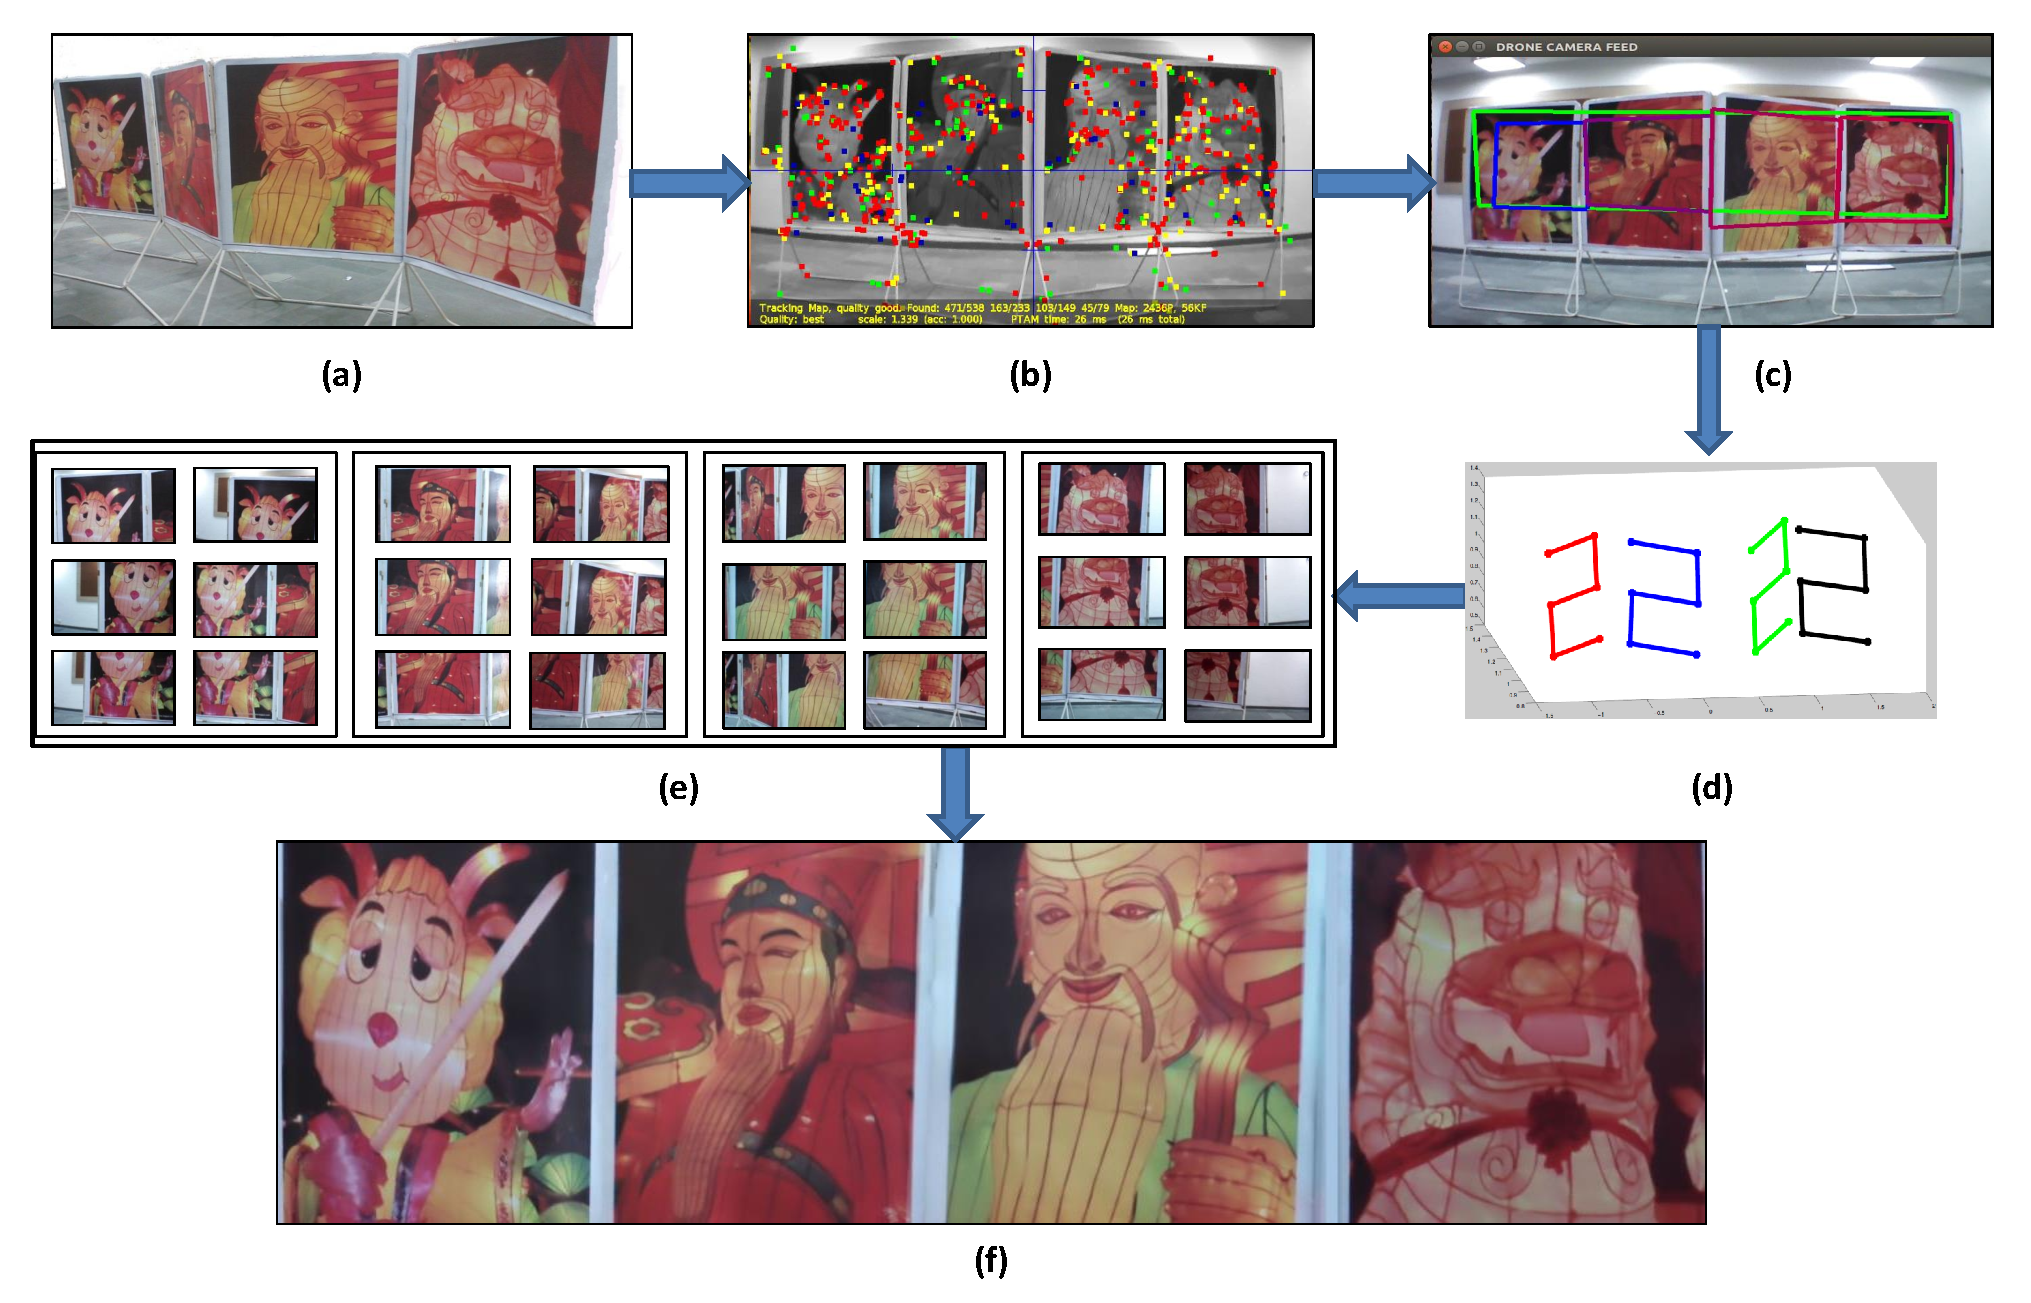
\includegraphics[width=\textwidth]{figures/multiplanar/workflow}
\caption[Overall Workflow]{Overview: (a) Input Scene to be imaged. (b) Feature
points in the scene are found and their 3D positions are estimated using scale aware PTAM \cite{engel}. (c) Multiple planar bounded
regions are estimated using our algorithm. (d) For each bounded planar region, 3D camera positions
are calculated and overall path planning is done. (e) Videos are captured at
each target position. From each captured video, the appropriate frame is
found. (f) Individual mosaics are joined together to get final output.}
\label{fig:workflow}
\end{figure}
\subsection{3D map}
We have used PTAM based method \cite{engel} to localize quadcopter as well as to
create a 3D map of surrounding environment (See Figure \ref{fig:ptam_output}).
In PTAM, initially, the prior pose is estimated using motion model. Then the map
points are projected into the image using prior pose estimate. Next, the camera
pose is updated using some of the feature matches in the image. Final pose
estimate is computed from all the matches found.
 
The initial map built from stereo initialization algorithm has an arbitrary
scale. Hence, there is need of scaling map to metric units. This is done by
assuming that the camera is translated 10 cm between the stereo pair. This
assumption may not be true in the case of inexpensive quadcopter due to its jerky
motions. So, proper scale estimation is necessary.

\textbf{Scale Estimation}
The quadcopter measures distance traveled during translation using PTAM as well as
available metric sensors (ultrasound altimeter) at regular intervals. We get
a pair of samples $\mathbf{x}_i, \mathbf{y}_i \in {\Re}^d$ where $\mathbf{x}_i$ is
scaled translation calculated from PTAM system and $\mathbf{y}_i$ is the distance
measured by the metric sensor at each interval. These pair of samples are related
according to $\mathbf{x}_i \approx \lambda \mathbf{y}_i$. The scale $\lambda$ is
estimated by minimizing the negative log-likelihood\cite{engel}.  

We could get the correct pose by  scaling  PTAM estimated pose. But we
cannot rely only on PTAM for pose estimation as visual feedback may lag due to
problems in wi-fi connectivity. Hence there is need of  alternative
mechanism as a fallback to PTAM. Engel et al. \cite{engel} have used Extended
Kalman Filter to fuse odometry observation model with visual observation model for state prediction i.e.,
estimating the pose (x,y,z and roll-pitch-yaw) of quadcopter at given  instant.

\textbf{State Prediction and Observation:} The state space consists of a total
of ten state variables. 
\begin{ceqn}
\begin{align}
	\mathbf{x}_t &\coloneqq {(x_t, y_t, z_t, \dot{x_t}, \dot{y_t},
	\dot{z_t}, {\Phi}_t, {\Theta}_t, {\Psi}_t, \dot{{\Psi}_t} )}^T  \in
	{\mathbb{R}}^{10},
\end{align}
\end{ceqn}
where $(x_t, y_t, z_t)$ represents the position of the quadcopter in
metric units and $(\dot{x_t}, \dot{y_t}, \dot{z_t})$, the velocity in m/s, both
in world coordinates. The state also contains three angles, i.e., the roll
${\Phi}_t$, pitch ${\Theta}_t$ and yaw ${\Psi}_t$ of the drone in degrees.  An observation
function $h(x_t)$ for each sensor as well as respective observation vector $z_t$
composed from the sensor readings is defined for each observation model.

\textbf{Odometry observation model:} Quadcopter measures its horizontal speed
(i..e., along x and y direction) in its local coordinate system which is
transformed into global coordinate system to get $\dot{x_t}$ and $\dot{y_t}$.
The roll and pitch angles are directly taken from the accelerometers'
observations. Height measurements ($\hat{h_t}$) and yaw measurements
($\hat{{\Psi}_t}$) are differentiated and treated as observations of respective
velocities. The resulting observation function $h_I(\mathbf{x}_t)$ and
measurement vector $\mathbf{z}_{I,t}$ is given by,
\begin{ceqn}

\begin{align}
	h_I(\mathbf{x}_t) &\coloneqq  
	\begin{pmatrix} 
		\dot{x_t}\cos{{\Psi}_t} - \dot{y_t}\sin{{\Psi}_t} \\
		\dot{x_t}\sin{{\Psi}_t} + \dot{y_t}\cos{{\Psi}_t} \\
		\dot{z_t} \\
		{\Phi}_t \\
		{\Theta}_t \\
		\dot{{\Phi}_t}   	
	\end{pmatrix}
	\\
	\mathbf{z}_{I,t} &\coloneqq (\hat{v}_{x,t}, \hat{v}_{y,t}, (\hat{h}_t -
	\hat{h}_{t-1}), \hat{{\Phi}_t}, \hat{{\Theta}_t}, (\hat{{\Psi}_t} - \hat{{\Psi}}_{t-1}  ) )^T
\end{align}
\end{ceqn}
\textbf{Visual Observation Model:} The pose estimate is scaled by the
current estimate for the scaling factor ${\lambda}^{*}$ when PTAM tracks a
video frame successfully. This pose estimate is transformed from the coordinate
system of the front camera to the coordinate system of the quadcopter. Direct
observation of the quadcopter’s pose is given by,
\begin{ceqn}

\begin{align}
	  h_P(\mathbf{x}_t) &\coloneqq  {(x_t, y_t, z_t, {\Phi}_t, {\Theta}_t,
	  {\Psi}_t)}^T \\
	  \mathbf{z}_{I,t} &\coloneqq
	  f(\mathbf{E}_{\mathit{DC}}\mathbf{E}_{\mathit{C},t} )
\end{align}
\end{ceqn}

where $\mathbf{E}_{\mathit{C},t} \in SE(3)$ is the estimated camera pose (scaled
with $\lambda$ ), $\mathbf{E}_{\mathit{DC}} \in SE(3)$ the constant
transformation from the camera to the quadcopter coordinate system, and $f :
SE(3) \rightarrow \mathbb{R}^6$ the transformation from an element of $SE(3)$ to
our roll-pitch-yaw representation.

\textbf{Prediction Model:} Extended Kalman filter is used to fuse all state
variables from both observation models. (Please see \cite{engel} for the
details). Finally prediction model describes how state vector $\mathbf{x}_t$
evolves from one time step to next. The quadcopter’s horizontal acceleration is
approximated $\ddot{x}, \ddot{y}$ based on its current state $\mathbf{x}_t$.
Quadcopter's vertical acceleration   $\ddot{z}$, yaw-rotational 
acceleration $\ddot{{\Psi}_t}$ and the roll/pitch rotational speed
$\dot{{\Psi}_t}, \dot{{\Theta}_t}$ is estimated based on the state
$\mathbf{x}_t$ and  active control command $\mathbf{u}_t$. Finally, using quadcopter's 
estimated pose information, we update the 3D map of the environment.

\noindent\textbf{Scale Accuracy:} 
Though \cite{engel}  gives 3D map of the environment, the scale accuracy is not
ensured. It may lead to inaccurate 3D coordinates of the feature points. To
ensure scale is 100 percent accurate, we moved the quadcopter autonomously in
the vertical direction (up and down) by fixed distance. The reason behind moving in
the vertical direction is that the sonar gives us very accurate height information 
which is used to remove scale ambiguity.

We have conducted a small experiment to demonstrate the efficacy of our method to
achieve 100\% scale accuracy. First, we initialized PTAM after
taking off the quadcopter, moved the quadcopter to location (0, 0, 1) i.e., 1
meter above ground, and finally landed it from the same location. Ideally,
take-off location and land location should be same. However, due to errors in
PTAM initialization as well as noise in IMU measurements, the distance between
two locations will be non-zero. We use this distance as a measure of error. We also tried to imbalance the quadcopter, while it is at location (0, 0, 1), before landing to check its
ability to come back to original position.

Later, we repeated the experiment with one change, instead of using only PTAM
initialization, we have autonomously moved the quadcopter up and down by fixed
distance (1 meter) after PTAM initialization. Our summarized observations
after ten runs in both cases are listed in Table~\ref{tab:ptamInit}.
\begin{table}
\centering
\newcolumntype{C}{ >{\centering\arraybackslash} m{2cm} }
\newcolumntype{D}{ >{\centering\arraybackslash} m{5cm} }
\begin{tabular}{|D|C|C|C|C|}
\hline
Case & Avg. Scale Accuracy & Avg. Scale (in m) & Number of Iterations &
Mean Error $\pm$ std. (in cm)\\
\hline
Only PTAM initialization & 0.524 & 1.2 & NA & 82.6 $\pm$ 10.73 \\
\hline
PTAM initialization with accuracy check & 1.0 & 2.33 & 3--4 & 13.2 $\pm3.6$\\
\hline       
\end{tabular}
\caption[Effect of ensuring scale accuracy on pose estimation]{Effect of
ensuring scale accuracy on pose estimation of quadcopter.
The first row shows that with only PTAM initialization, we do not get the accurate pose.
When we use our method to ensure the 100\% scale accuracy, we are much better in
pose estimation. The scene used for this testing was 2.3 meters away from the
quadcopter. As the estimated scale (2.33m) with our method is very close to the
actual distance of the scene from a quadcopter, generated 3D map will be also very
accurate.}
\label{tab:ptamInit}
\end{table}
Table~\ref{tab:ptamInit} clearly indicates that the pose estimate with only PTAM
initialization is far off (around 85cm) from actual position\footnote{We also
noted that sometimes quadcopter was not able to come anywhere near to (0, 0, 1)
if we imbalance a quadcopter purposefully after PTAM initialization.}.
However, when we ensure scale accuracy the estimated pose is within 15 cms of the
actual location. The estimated scale is also very close to the actual distance of
the plane, if we use our method for ensuring 100\% scale accuracy.

\begin{figure}[t!]
\centering
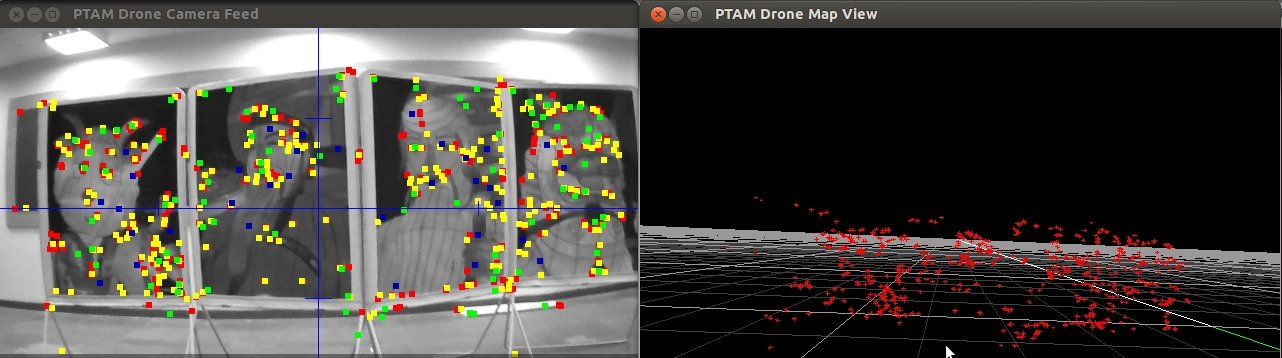
\includegraphics[width=\linewidth]{images/3D_2D}
\caption[Creation of 3D map]{Mapping of 3D locations to 2D image pixel locations
of feature points using PTAM. Left: Camera view showing 2D locations of detected feature points.
Color coding indicates the coarseness level of detected features. Right: Mapview
showing 3D locations of detected feature points.}
\label{fig:ptam_output}
\end{figure}

\subsection{Human Interaction}
Next step after we get a 3D map of the environment is getting the desired area for
imaging from the user. The user may be interested in a scene spread over multiple
planes. Also, the user would like to cover a particular part of it. So we need
to identify the area of interest of the user on the multiplanar surface.
Hence, we  first fly the quadcopter at a sufficiently far distance from the
surface. The distance should be such that the user can see the whole
scene.We have created a user interface which enables the user to mark the region
of interest.\\
\begin{figure}[t!]
\centering
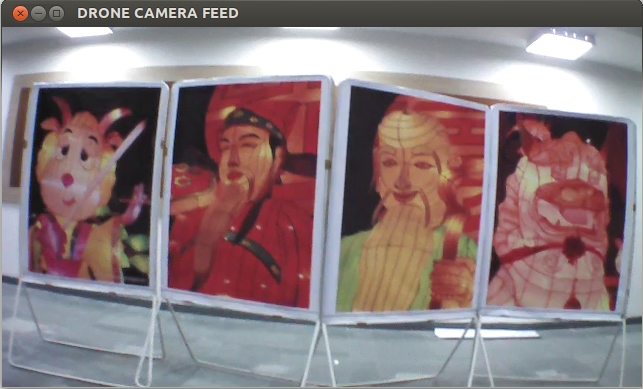
\includegraphics[width=0.31\linewidth]{images/UI_input}
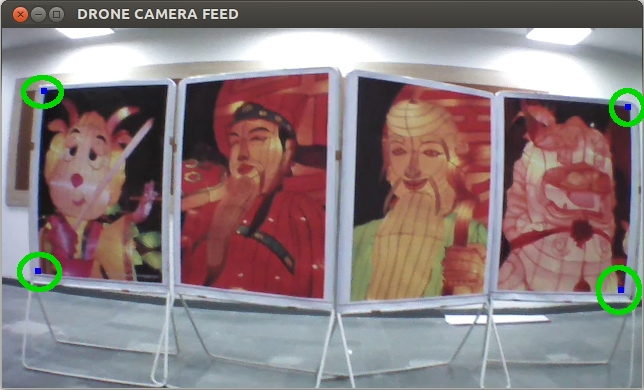
\includegraphics[width=0.31\linewidth]{images/UI_points_marked}
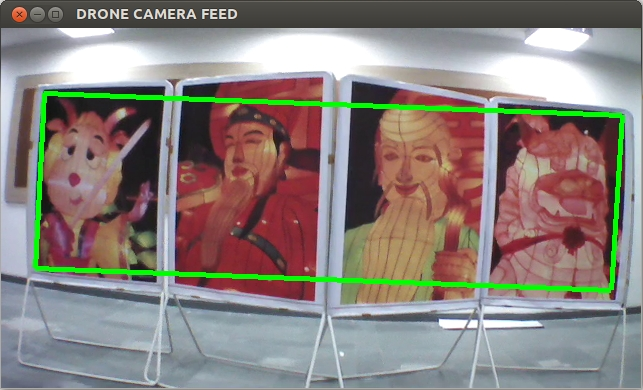
\includegraphics[width=0.31\linewidth]{images/UI_convexHull}
\caption[Our user interface]{Left: The user is shown a live video stream as seen
from a quadcopter camera. Middle: The user may click points to denote the area of interest. We 
find out the nearest 3D point and show its projection (encircled blue pixels) on
the image plane. Right: Once user finishes with clicking points, we find out its convex
hull and show it in green convex polygon.}
\label{fig:ui}
\end{figure}
\textbf{User interface} User is shown the live video stream as seen through
the quadcopter (Figure \ref{fig:ui}(Left)). Now, users can click points to
mark their area of interest on the 2D screen. At backend we determine the
nearest 3D point corresponding to the location clicked by the user and then show
its projection on the image plane. (Figure \ref{fig:ui}(Middle)). Once they
finish with marking the points, they can see the convex hull of the
clicked points in order to check the area to be covered is indeed the area of
interest (Figure \ref{fig:ui}(Right)). The user can optionally add or delete points
or even completely remove all clicked points using the interface.

\subsection{Multiplanar Regions Detection}
We need to detect multiple planes present in the user's region of
interest. There are many algorithms such as Sequential RANSAC\cite{Kanazawa},
multiRANSAC\cite{zuliani} , J-linkage\cite{jlinkage}, T-linkage\cite{tlinkage}
etc. to detect multiple models from the data. But we have chosen real-time
implementation of J-linkage \cite{realtimejlinkage}.\\
\textbf{J-linkage:} Sequential RANSAC and multiRANSAC algorithms require
the number of planes as an input parameter. But as the number of planes changes
according to the input scene, we cannot use these algorithms. J-Linkage and T-Linkage
doesn't require the number of planes as an input parameter. 
%Though T-Linkage is more robust to noise in the input points, it is an order of
%magnitude slower than J-Linkage. 
In our application, detection of the number of planes is the first and most
important step. Hence it needs to be done in real-time which makes J-Linkage
more suitable than T-linkage.

But J-Linkage doesn't give the extent of the plane, i.e., bounded
region. It tries to fit all points to the planes. Figure \ref{fig:multiplane}
depicts the relevant scenario. As we can see, there are some points which may
be the result of inaccurate 3D map generated by PTAM (indicated by a black oval).
As these points have ``geometric'' affinity towards plane A, J-linkage puts these
points in plane A\textquotesingle s cluster. But in the real world, they are part
of plane B.
So we need to disambiguate such points for correct calculation of multiplanar
bounded regions. We have developed an algorithm to modify the output of
J-Linkage to give correct bounded multiplanar regions.\\
\textbf{Improvement over J-Linkage:} JLinkage algorithm output label
for each data point denoting to which plane that data point belongs to. Our
algorithm does following to find continuous multiplanar bounded regions from J-Linkage
output.
\begin{itemize}
  \item Run clustering algorithm e.g., k-means using the output of J-linkage
  as initial labels.
  \item Find out the distance of all points inside each cluster from the cluster
  centroid along the normal of the given plane.
  \item Remove the points from the cluster which are more than 95 percentile
  farther from the cluster centroid along the plane normal.
  \item Find out the bounding rectangle of each cluster.
  \item Extend the rectangle till the intersection with the successive plane.
\end{itemize}

This process is illustrated in Figure \ref{fig:multiplane}. JLinkage
gives us the labeling according to each point's vicinity to the detected
planes. But the 3D points estimated by PTAM may be erroneous due to noise,
marked by circles in Figure \ref{fig:multiplane}(Top). As these points do not
belong to the planes labeled by JLinkage, it gives us wrong bounded
regions. So, we run k-means algorithm using the initial labels given by
JLinkage. Now, points  belong to the correct cluster as shown in
Figure \ref{fig:multiplane}(Middle). But, we don't want points which are far
away from the plane in a normal direction. Hence we remove those points which
are more than 95 percentile farther from the cluster centroid along the plane
normal. We also trim the boundaries of a plane by the bounding box of the
enclosed points. The final output is shown in the Figure
\ref{fig:multiplane}(Bottom).

\begin{figure}[h!]
\centering
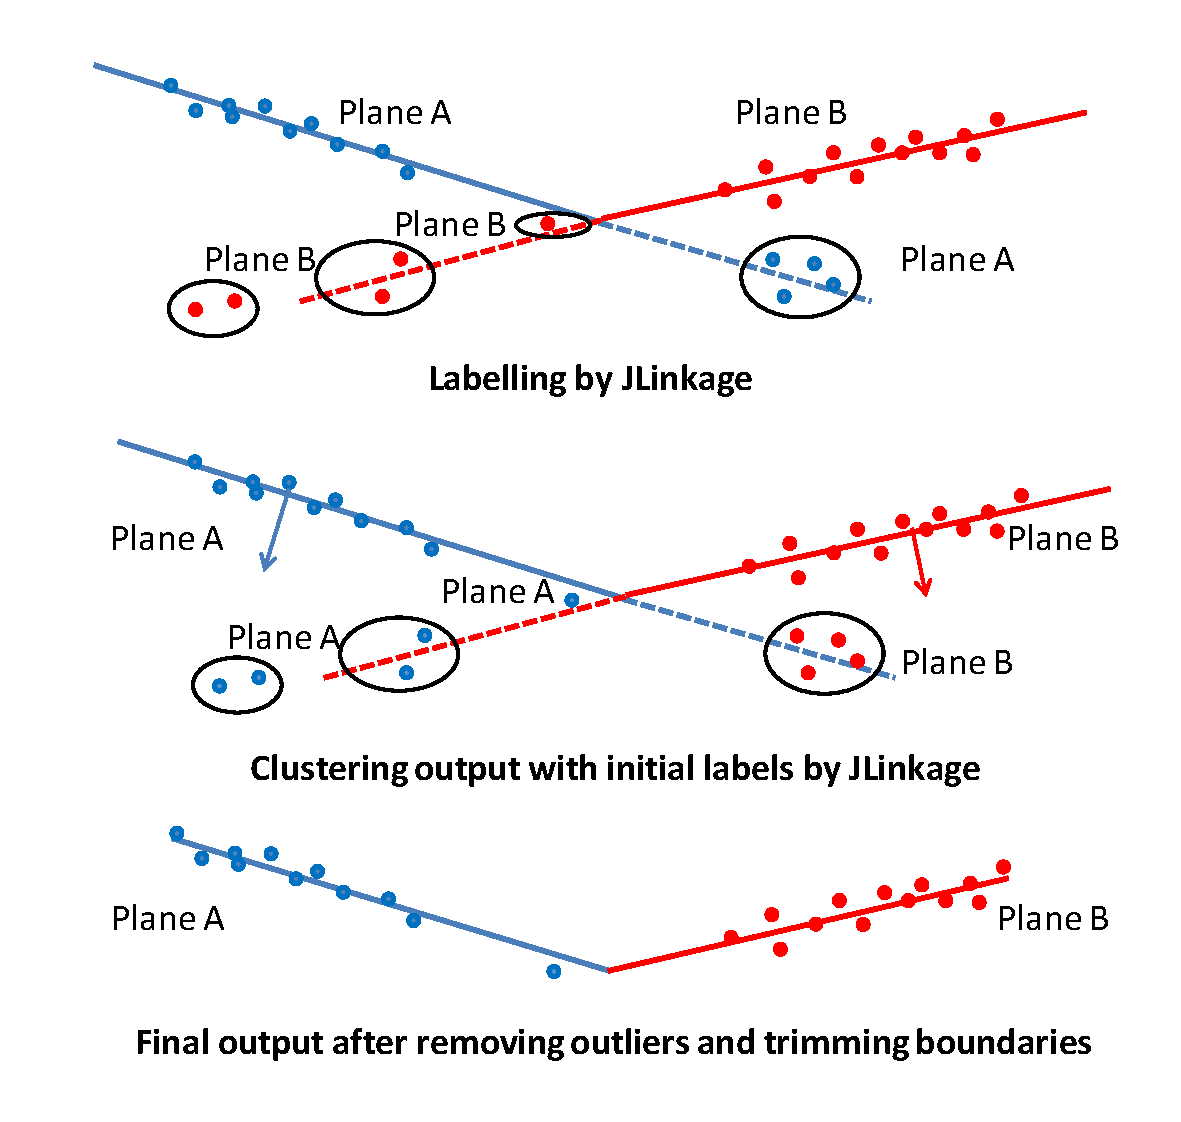
\includegraphics[width=\linewidth]{figures/multiplanar/multiplaneDetection}
\caption[Multiple planes detection]{Process of finding multiplanar bounded
regions from JLinkage output.
The top image shows us the initial labeling given by JLinkage. Later we run a
k-means algorithm using initial labeling given by JLinkage. The output is shown
in the middle figure. Finally, we remove outliers which are farther from the
plane along normal direction and trim boundaries of the plane as shown in
the bottom figure.}
\label{fig:multiplane}
\end{figure}

Each bounded planar region is used to determine the path along which
the quadcopter is navigated to cover that region.

\subsection{Path Planning}
The bounded region is divided into a grid of overlapping cells as shown in
Figure \ref{fig:grid}. We intend to cover each cell in a single image and then
use images from all cells to create a mosaic of given bounded planar
region. Cell area (width, height) is decided on the basis of the amount of details required of the
scene. E.g., if we need to probe our scene with minute details, we have to go
nearer to the plane. So, in that case, cell area is smaller. We need
overlap between neighbor images for successful mosaicing. So, the amount of
overlap between two cells is a function of the required overlap in feature space
needed for stitching. Currently, the overlap is set at thirty percent of cell area to deal
even with sparser (containing fewer feature points) images. Once we
calculate coordinates of cell corners, we determine the desired position of
a camera from where the whole cell area is covered in a single image. We repeat
this process for each cell to find out the path of quadcopter to cover the region in
optimal (in a number of positions) manner so that whole region is covered.

\begin{figure}[h!]
\centering
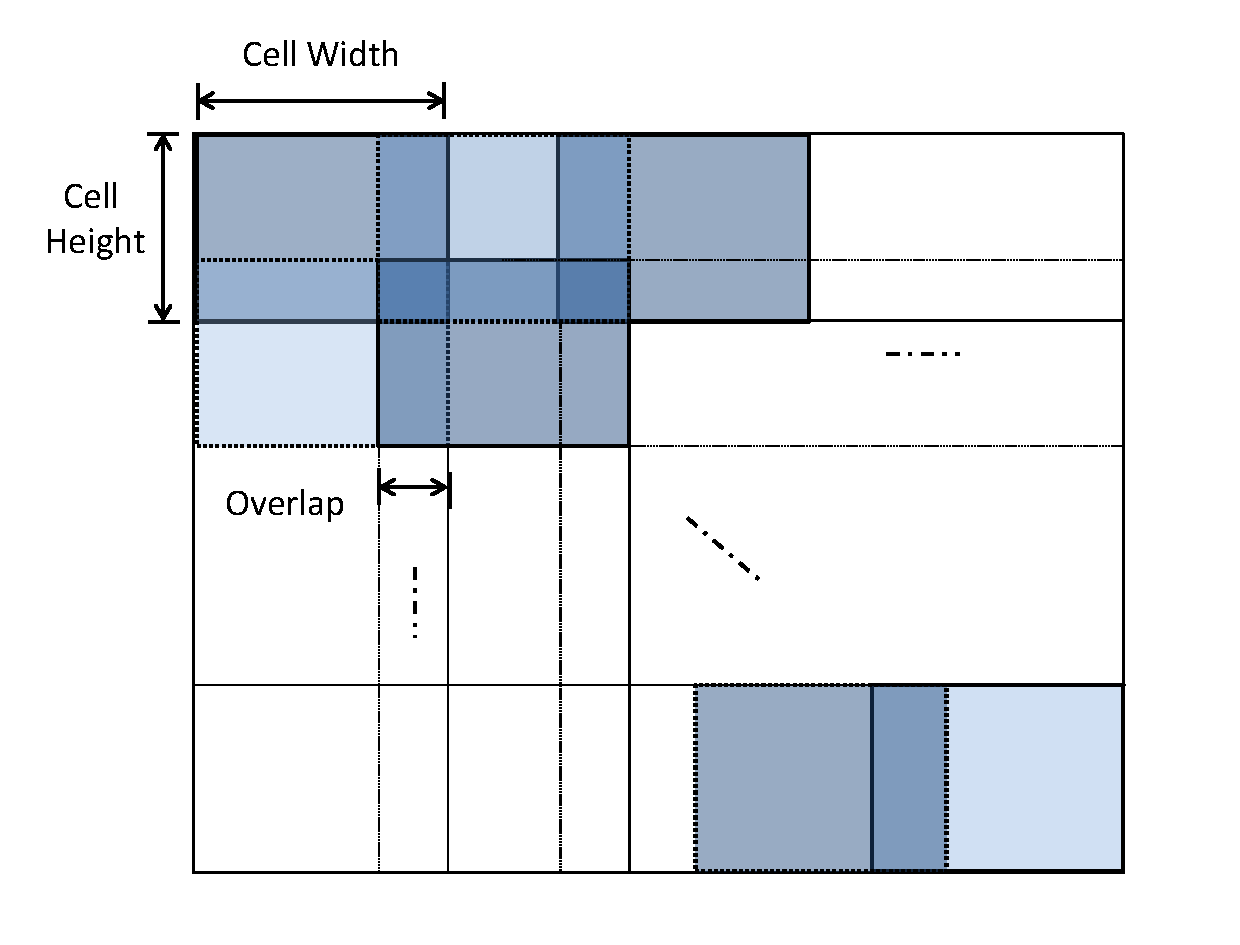
\includegraphics[width=\linewidth]{figures/multiplanar/PathPlanningGrid}
\caption[Path planning]{Grid of overlapping cells designed for path planning.
There is such grid for each planar bounded region. Cell Width and Cell Height is decided based
on the area we would like to capture in one frame. Overlap parameter is
a function of overlap required in feature space for successful stitching.
We find camera position for each cell in the grid which in turn
gives us the path for quadcopter to cover the given planar bounded region.}
\label{fig:grid}
\end{figure}

\subsection{Navigation of a quadcopter}
 We use the pose estimate provided by PTAM  based method \cite{engel}to track
 the quadcopter during navigation along the planned path.\\
\textbf{Covering a single planar bounded region}:
We navigate the quadcopter smoothly in a ``snake scan'' manner along the target points estimated in path
planning step to cover each planar bounded region.\\
\textbf{Transition from one plane to another plane}: We make sure the
transition in terms of yaw as well as horizontal movement is smooth. In order to achieve this,
we divide the horizontal distance into three parts and  move along x and y-axis
alternatively. During each step, we change the yaw in equal proportion so that
the quadcopter’s view is not changed drastically which is very important for
tracking using PTAM \cite{engel}.

\subsection{Recording video and ROS streams}
%AR Drone doesn't have the capability of taking still photographs. 
 We are not sure about the exact position of a quadcopter while capturing
 images due to an error in PTAM as well as the jerky motion of quadcopter. So, we record a video on USB device onboard quadcopter for a small amount
 of time (3 seconds) when we are in proximity of the specified point calculated in path planning. We
also record ROS streams (image as well as navigation data) captured over Wi-Fi.\\
\textbf{Finding the sharp and exact image from video:} We need to find the sharp
image i.e., an image with the minimum blur which is closest to the target point
from 3 seconds HD video (approximately 90 images). But there is no positional data
available on USB device. Navigational data and image streams captured over Wi-Fi help us
in this process. First, we synchronize these two streams using timestamp
information. It gives us an approximate position of each image from the image
stream. Now we select the sharpest image among the images which are taken from
positions in a close proximity of the specified point. Later we match each
image from the HD video with the selected image from the image stream using SURF
features. And finally we select the sharpest image from the HD video among
all images (from the HD video) which are within a threshold in SURF\cite{Bay}
feature space from the selected image from the image stream.

\subsection{Creating mosaic of the multiplanar bounded region}
Once images for each planar bounded region are found from captured
videos, mosaic for each planar region is created using the method of creation of
a mini-panorama presented in \cite{Prasad16}. In \cite{Prasad16}, first images
are arranged in a rectangular grid according to their positions. Here, as we already have grid
information (created in path planning step), our first step is partially done.
Later, we do feature matching among the neighborhood images and create the
maximum spanning tree using  the homography inliers as weight. Finally, mosaic
i.e., mini-panorama is created by warping images according to the respective
homography matrix (w.r.t. the  reference image).

After the creation of mini-panorama for each planar region, we join all
mini-panoramas using a method similar to the creation of super panorama used in
\cite{Prasad16}. In \cite{Prasad16}, the super-panorama is created by finding the
disparity between the reference images of each mini-panorama using the distance
between the camera and the imaging plane and, camera positions of reference
images for each mini-panorama. As all mini-panoramas were in the same plane,
simple stereo formulation (without rectification) was enough. In our case, as
mini-panoramas belong to multiple planes, we need to make sure that all
mini-panoramas are in the same plane to find the disparity among reference images of
 all mini-panoramas, which requires image rectification. But, as we keep the
 quadcopter's camera normal to the plane while capturing reference image for each
 mini-panorama, we don't have to do full rectification.
 We just need to calculate the distance between the center of projections, projected on the imaging plane, 
 along the planes as shown in Figure \ref{fig:multiplanarMosaic}.

\begin{figure}[ht!]
\centering
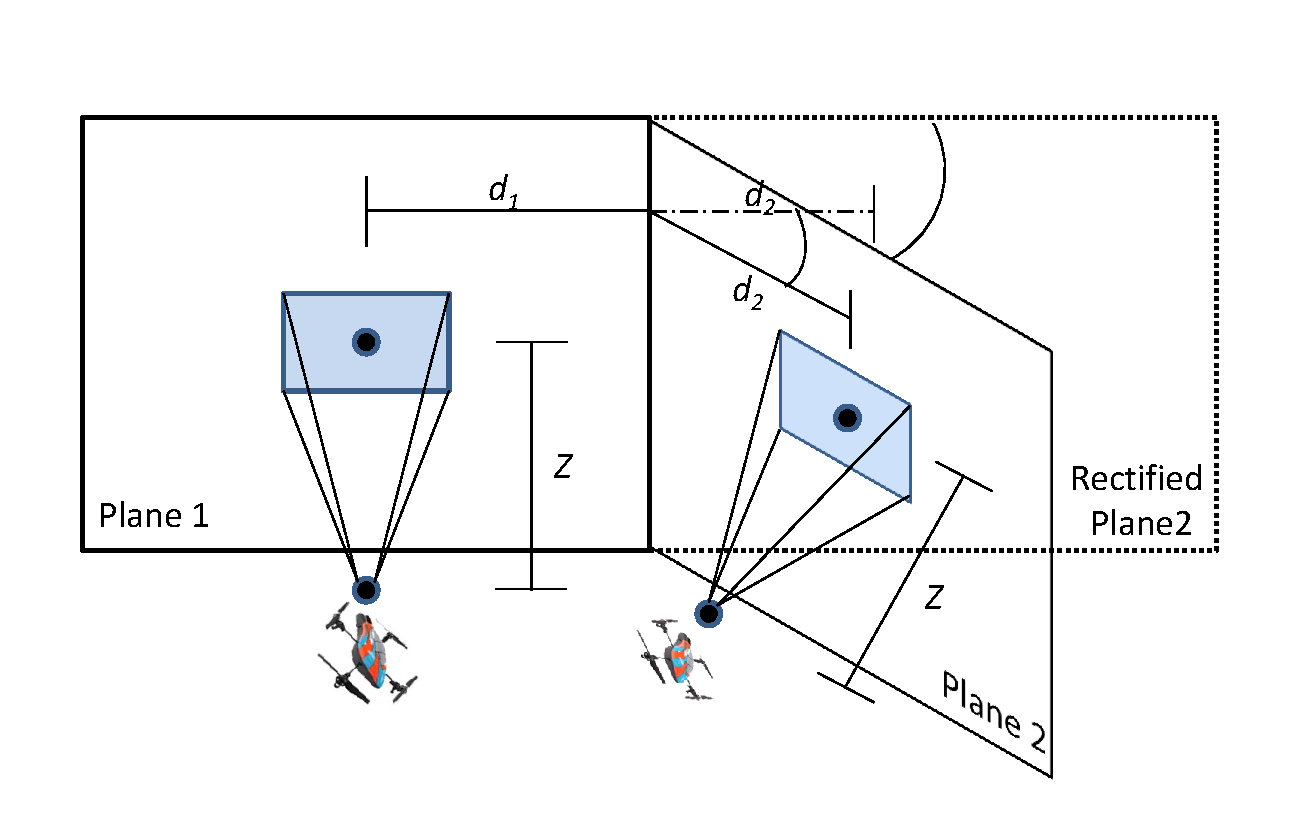
\includegraphics[width=\linewidth]{figures/multiplanar/MultiplanarMosaic}
\caption[Super panorama for multiplanar scene]{Process of finding disparity
between reference images of mosaics imaged on two different planes.}
\label{fig:multiplanarMosaic}
\end{figure}

Let us assume that the depth of the camera from both imaging planes is same
(say $Z$). Now, the disparity of image on the second plane with respect to the
image on the first plane is given as follows\cite{Prasad16}:
\begin{ceqn}
\begin{align}
\textit{disparity} = \textit{focal length}\frac{(d_1+d_2)}{Z}
\label{eq:disparity}
\end{align}
\end{ceqn}

where $d_1$ and $d_2$ are distances of back-projections of the center of
projections on the first and second plane respectively from the line of
the intersection between two planes and $Z$ is the distance between the center of
projection and the plane.

If center of projections are at different depths (e.g., say $Z_1$ and
$Z_2$), first we bring the image at lesser depth (say $Z_1$) to the same depth
of another image (which is imaged at larger depth, say $Z_2$) by zooming out by
fraction $\frac{Z_1}{Z_2}$. Later, we use Eq. \ref{eq:disparity} to calculate
the disparity by setting $Z=Z_2$.

\section{Experiments and Results}
All our experiments have been completed with the inexpensive consumer
quadcopter called  Parrot’s AR Drone 2.0. The camera resolution of AR Drone 2.0
is 1280 $\times$ 720\footnote{But when we stream the image over Wi-Fi the resolution
of an image is 640 $\times$ 360.}. We have used ROS based ARDrone Autonomy
Driver to communicate with the drone. For the purpose of showing the efficacy
of our method, we also took a picture of the scene from a distance with a 5
mega-pixel camera to better understand the scene. We have implemented our
algorithm in C++ using the OpenCV library (OpenCV 2.4.9).  Experiments were
performed on a laptop with Intel Core i5 processor(@2.4GHz) and 8GB RAM.

\subsection{Single Plane with Multiple Visits}
We have first used our algorithm to image a single planar wall shown in
Figure \ref{fig:resultLady}(Left). As the wall was too tall and it was not
possible to see the complete wall in one flash due to a shortage of space, we selected the
desired area in two steps as shown in Figure  \ref{fig:resultLady}(Middle). In path planning 37 (12
for the top and 25 for the bottom) positions were estimated to cover full region. Images
captured from those positions are mosaiced using our algorithm to get final
mosaicing output as shown in Figure \ref{fig:resultLady}(Right).

\begin{figure}
\centering
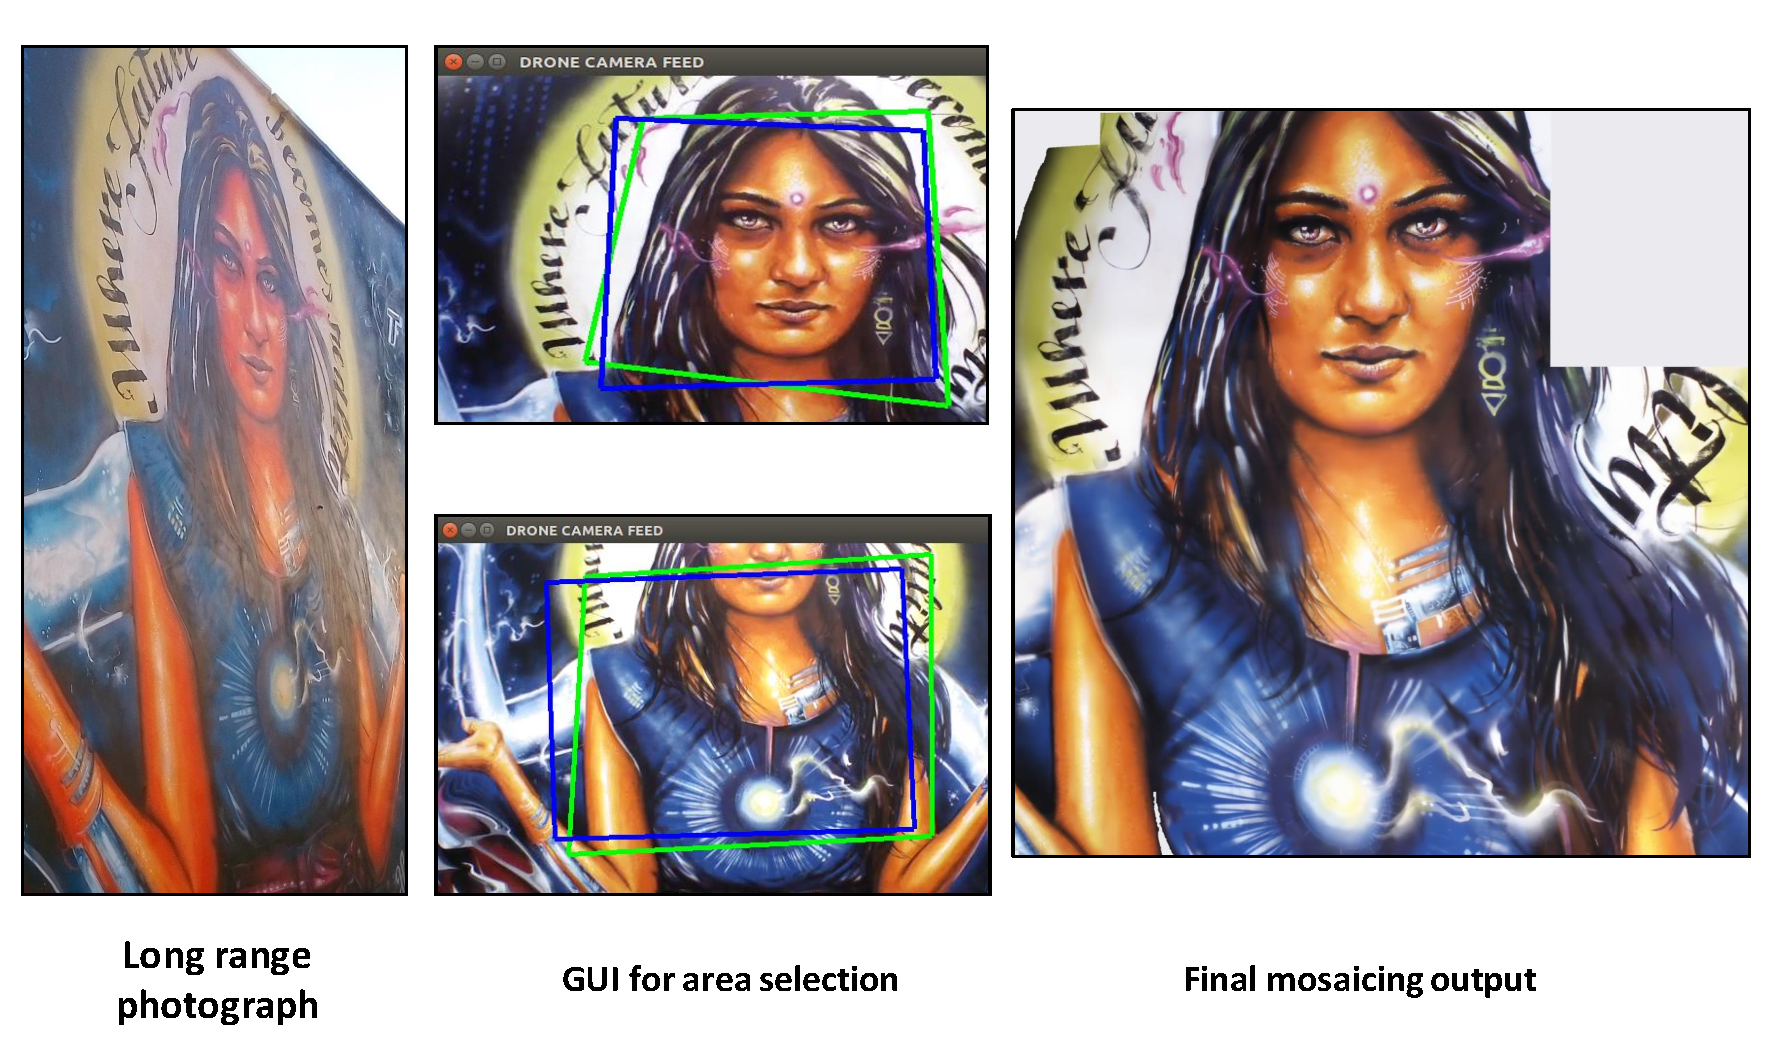
\includegraphics[width=\linewidth]{figures/multiplanar/ladyResult.pdf}
\caption[Result: Single planar scene]{There is a 15 feet tall wall as shown in
the long range photograph (left) which we would like to cover orthographically and with details. We cannot
select the whole area in a single instance as we cannot go back to see the whole
wall. Hence, we selected the desired area in two steps as shown in GUI for area
selection (middle-top and middle-bottom). Green quadrilateral shows user selected area
while blue quadrilateral shows the planar bounded region estimated by our
algorithm. In path planning 37 (12 for the top and 25 for the bottom) positions were
estimated to cover the full region. Images captured from those positions are
mosaiced using our algorithm to get the final mosaicing output as shown in the
right image.}
\label{fig:resultLady}
\end{figure}

\subsection{Multiple Planes}
Our further experiments are done on various setups covering multiple planes.\\

\textbf{Concave:} In this experiment, the exhibits were arranged in the concave
fashion as shown in Figure \ref{fig:resultConcave}(Top-Left). We have selected
the area to be imaged as shown in Figure \ref{fig:resultConcave}(Top-Right). In
the path planning stage, overall 27 (9 from the left plane, 12 from the middle and 6
from the right plane) positions were estimated to cover full region. Images captured
from those positions are mosaiced using our algorithm to get the final mosaicing
output as shown in the Figure \ref{fig:resultConcave}(Bottom).

\begin{figure}
\centering
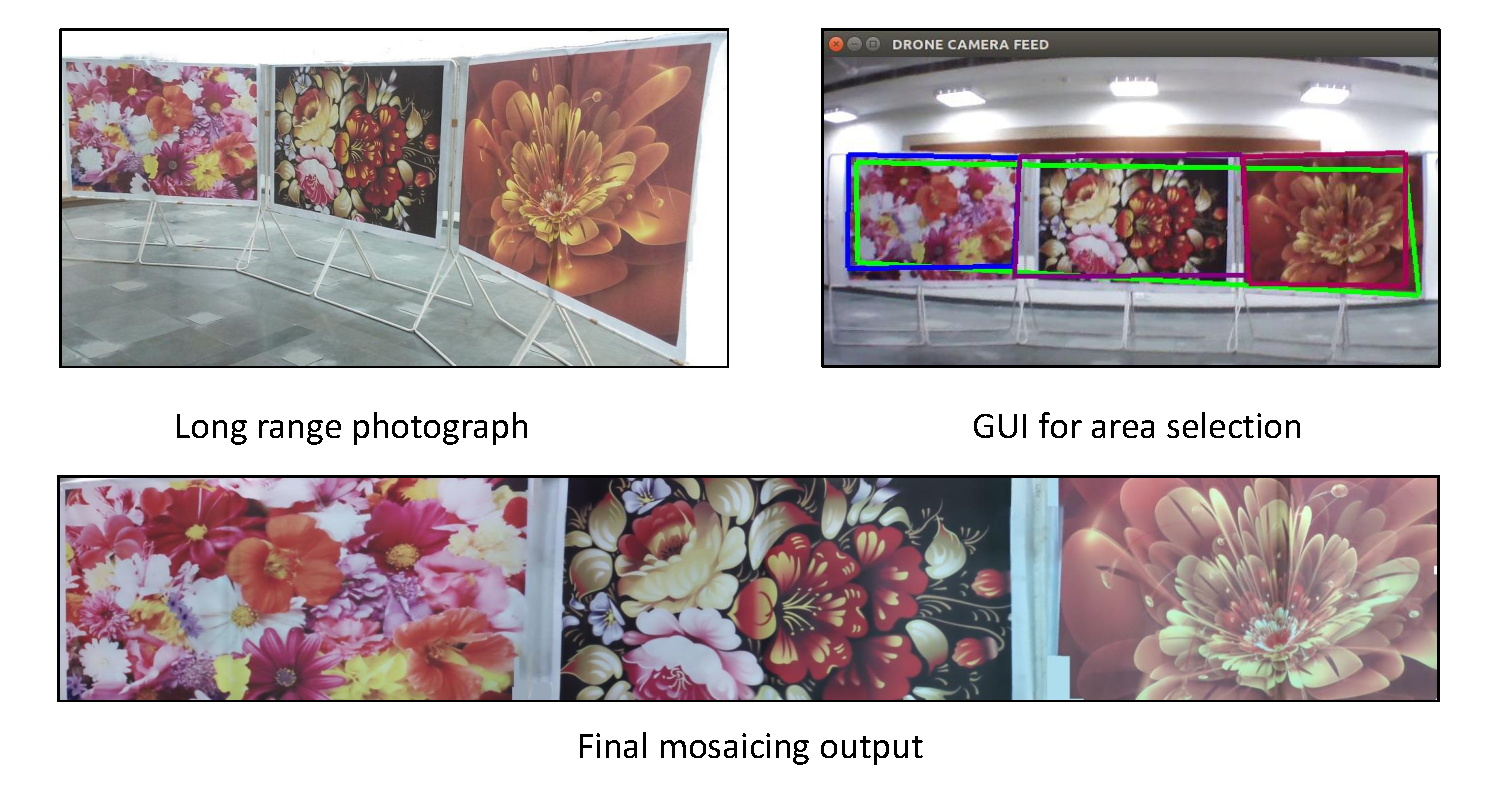
\includegraphics[width=\linewidth]{figures/multiplanar/ConcaveResult.pdf}
\caption[Result: Concave arrangement]{There is an art exhibition containing
multiple posters arranged in concave fashion as shown in the long range photograph (top-left). We have
selected the area to be imaged as shown in GUI for area selection(top-right).
Green quadrilateral shows user selected area while blue, violet and magenta
colored quadrilaterals represent the multiple planar bounded regions
estimated by our algorithm. In the path planning stage, overall 27 (9 from the left
plane, 12 from the middle and 6 from the right plane) positions were estimated to cover
full region. Images captured from those positions are mosaiced using our algorithm
to get the final mosaicing output as shown in the bottom image.}
\label{fig:resultConcave}.
\end{figure}

\textbf{Convex:} In this experiment, paintings were arranged in the convex
fashion as shown in Figure \ref{fig:resultConvex}(Top-Left). We have selected
the area to be imaged as shown in Figure \ref{fig:resultConvex}(Top-Right). In
the path planning stage, overall 30 (9 from the left plane, 12 from the middle and 9
from the right plane) positions to cover full region are estimated.  Images
captured from those positions are mosaiced using our algorithm to get the final
mosaicing output as shown in the Figure \ref{fig:resultConvex}(Bottom).

\begin{figure}[t!]
\centering
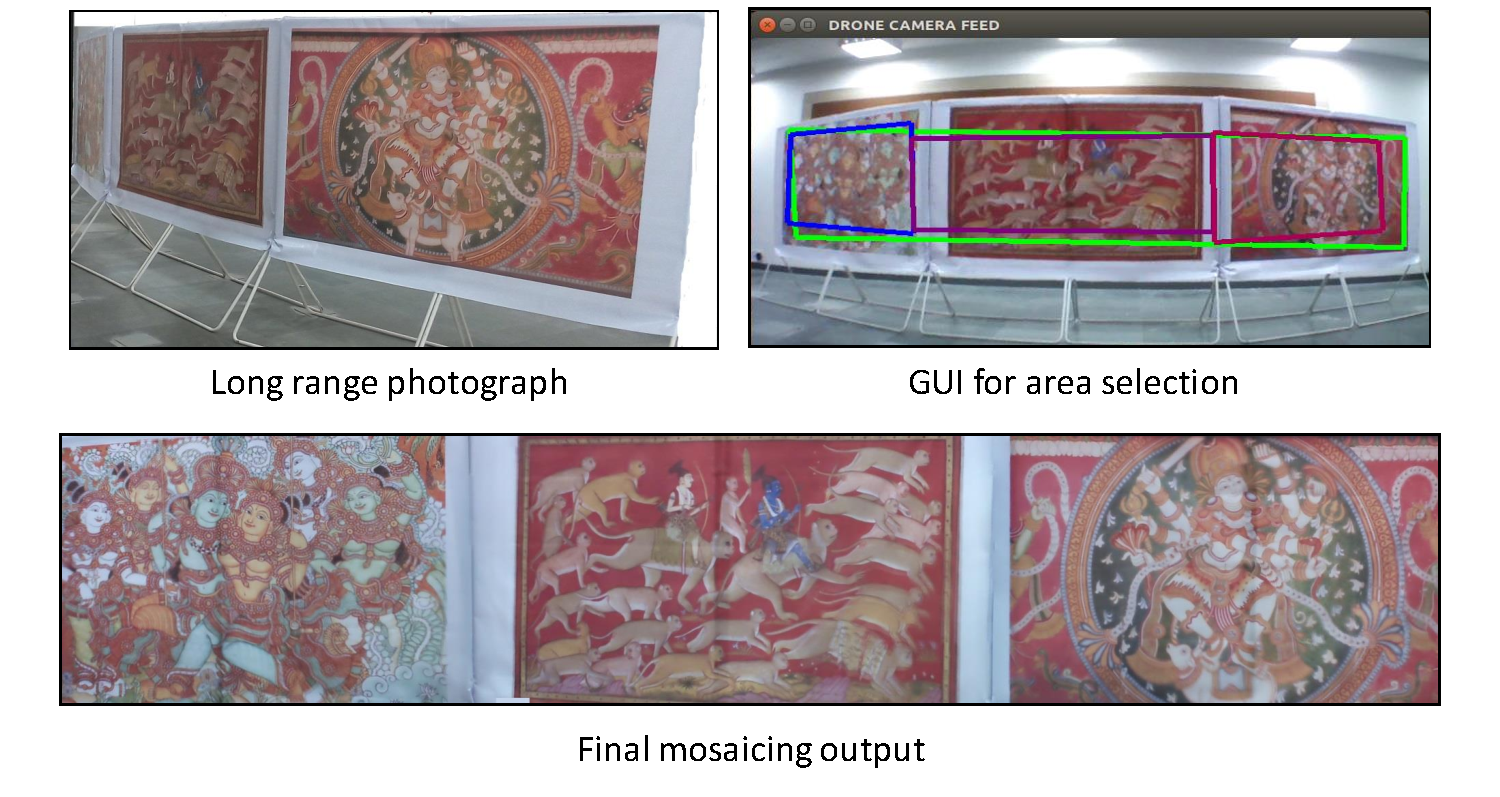
\includegraphics[width=\linewidth]{figures/multiplanar/convexResult.pdf}
\caption[Result: Convex arrangement]{There is an exhibition of Indian temple
paintings arranged in convex fashion as shown in the long range photograph (top-left). Note that we
cannot cover all paintings with enough details simultaneously. We have selected
the area to be imaged as shown in GUI for area selection (top-right).
Green quadrilateral shows user selected area while blue, violet and magenta
colored quadrilaterals represent the multiple planar bounded regions
estimated by our algorithm. In the path planning stage, overall 30 (9 from the left
plane, 12 from the middle and 9 from the right plane) positions were estimated to cover
the full region. Images captured from estimated positions are mosaiced using our
algorithm to get the final mosaicing output as shown in the bottom image.}
\label{fig:resultConvex}
\end{figure}

\textbf{Mixed:} We have performed a couple of experiments where posters were
arranged in mixed fashion. First arrangement looked like Figure
\ref{fig:resultMixed1}(Top-Left) where middle posters form convex region while
side posters form concave region. The selected area for imaging is shown in
Figure \ref{fig:resultMixed1}(Top-Right). In path planning overall 24 (6 from each
plane) positions are estimated to cover full region. Images captured from
those positions are mosaiced using our algorithm to get the final mosaicing
output as shown in the \ref{fig:resultMixed1}(Bottom).

\begin{figure}[t!]
\centering
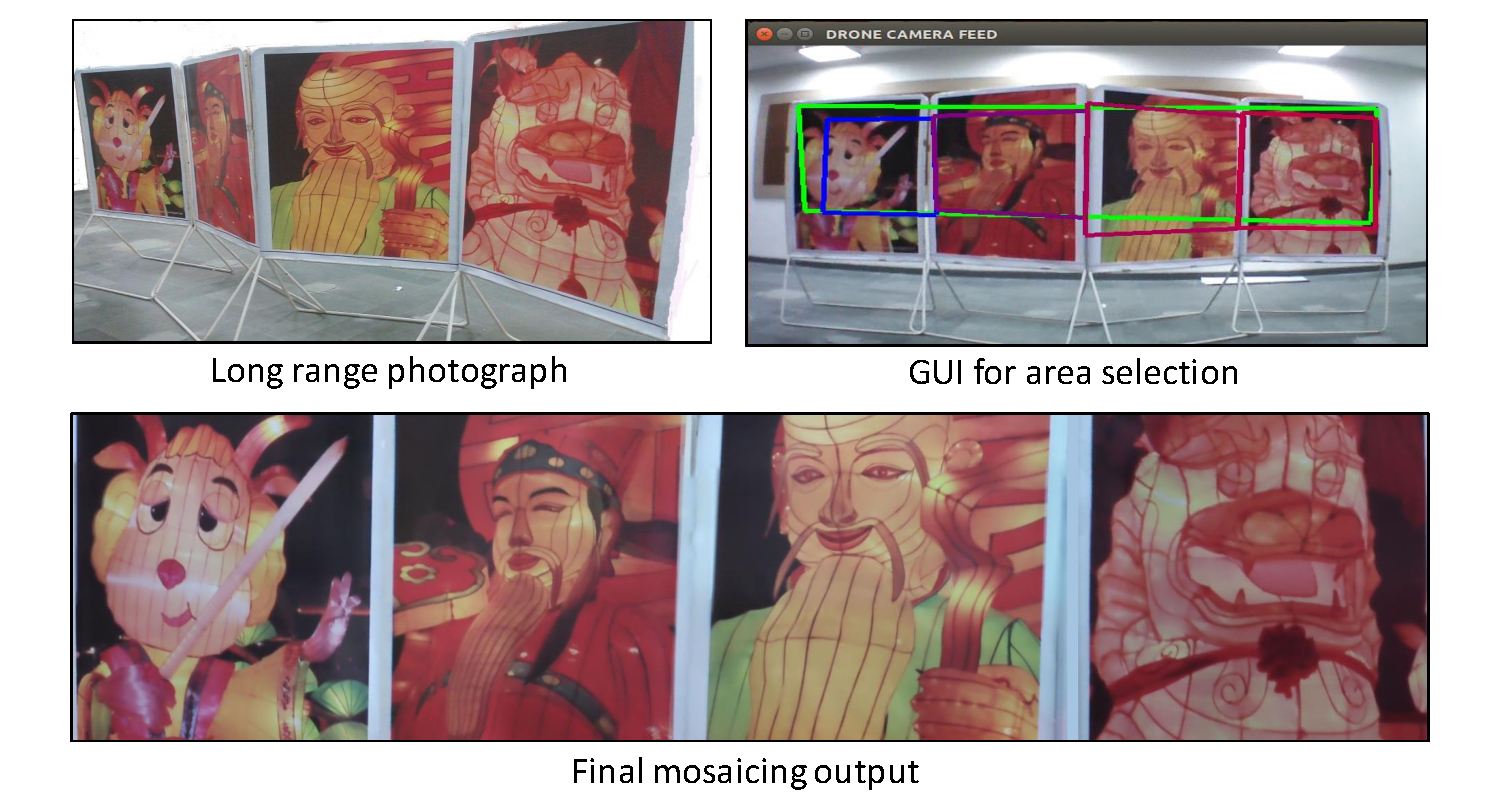
\includegraphics[width=\linewidth]{figures/multiplanar/mixed1Result.pdf}
\caption[Result: Mixed arrangement]{There is an exhibition of Chinese lanterns'
posters arranged in mixed (concave and convex) fashion as shown in the long range photograph
(top-left). Note that we cannot cover all paintings with enough details
simultaneously. We have selected the area to be imaged as shown in GUI for
area selection (top-right). Green quadrilateral shows user selected area while
blue, violet and magenta colored quadrilaterals represent the multiple
planar bounded regions estimated by our algorithm. In the path planning overall
24 (6 from each plane) positions were estimated to cover the full region. Images
captured from estimated positions are mosaiced using our algorithm to get the
final mosaicing output as shown in the bottom image.}
\label{fig:resultMixed1}
\end{figure}

In the second mixed arrangement, middle posters form concave region while
 side posters form convex region as shown in Figure
\ref{fig:resultMixed2}(Top-Left). The selected area for imaging is shown in
Figure \ref{fig:resultMixed2}(Top-Right).  In path planning overall 24 (6 from
each plane) positions were estimated to cover full region. Images captured from
estimated positions are mosaiced using our algorithm to get the final mosaicing
output as shown in the Figure \ref{fig:resultMixed2}(Bottom).

\begin{figure}
\centering
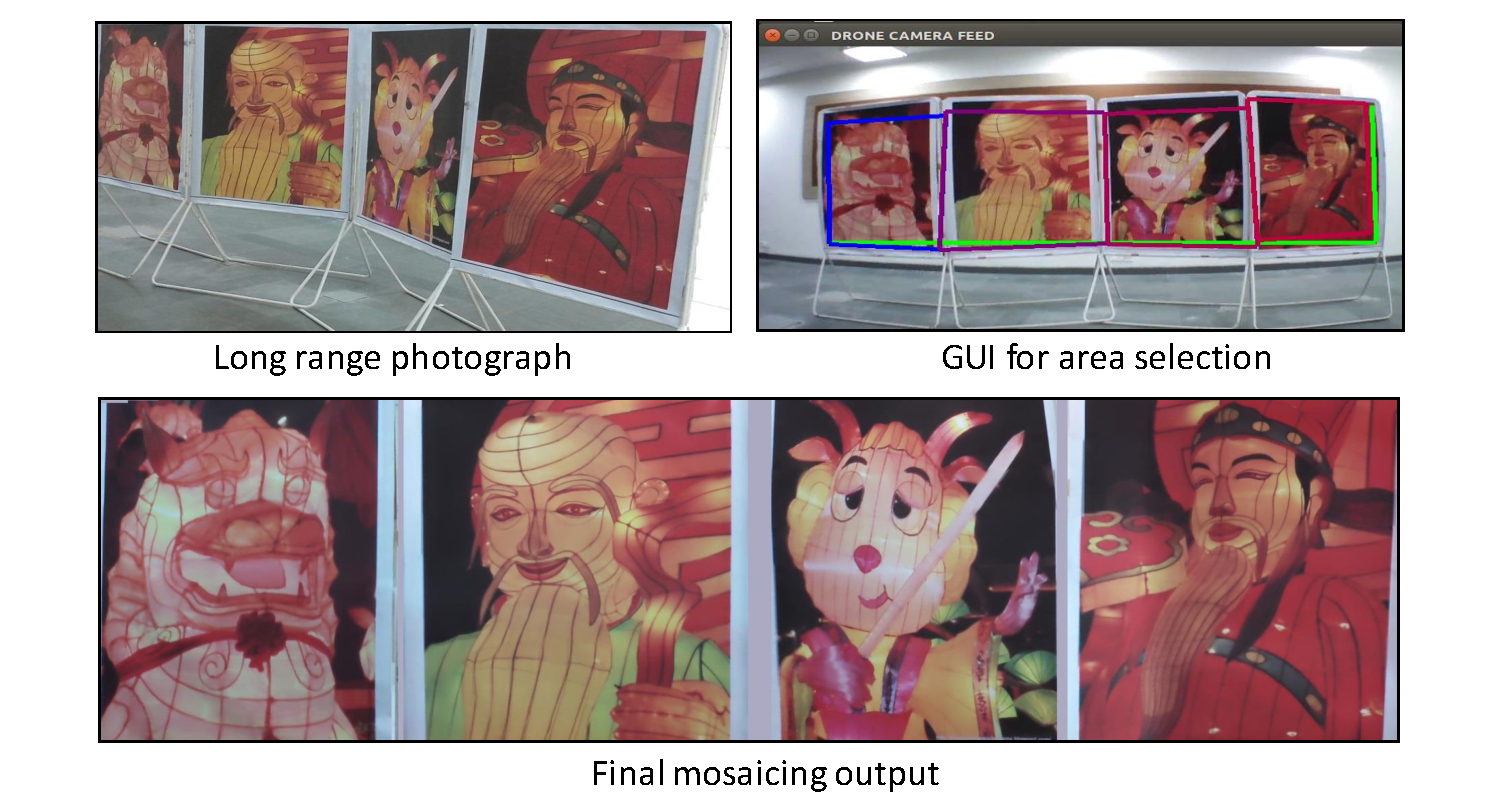
\includegraphics[width=\linewidth]{figures/multiplanar/mixed2Result.pdf}
\caption[Result: Mixed arrangement]{There is an exhibition of Chinese lanterns'
posters arranged in mixed (concave and convex) fashion as shown in the long range photograph
(top-left). Note that we cannot cover all paintings with enough details
simultaneously. We have selected the area to be imaged as shown in GUI for
area selection (top-right). Green quadrilateral shows user selected area while
blue, violet and magenta colored quadrilaterals represent the multiple
planar bounded regions estimated by our algorithm. In the path planning
stage, overall 24 (6 from each plane) positions were estimated to cover the full
region. Images captured from estimated positions are mosaiced using our
algorithm to get the final mosaicing output as shown in the bottom image.}
\label{fig:resultMixed2}
\end{figure}

\textbf{Planes at different depth:} In this experiment we have arranged posters
parallel to each other, but at different depths, as shown in Figure
\ref{fig:resultFrontBack}(Top-Left). It is not possible to mosaic them together
due to change in planes. But we have imaged each exhibit independently using
quadcopter and brought the mosaic of an exhibit at a larger depth to the same depth
of lesser depth exhibit mosaic using the estimated plane equations' information.
The final result is shown in the Figure \ref{fig:resultFrontBack}(Bottom).
\begin{figure}
\centering
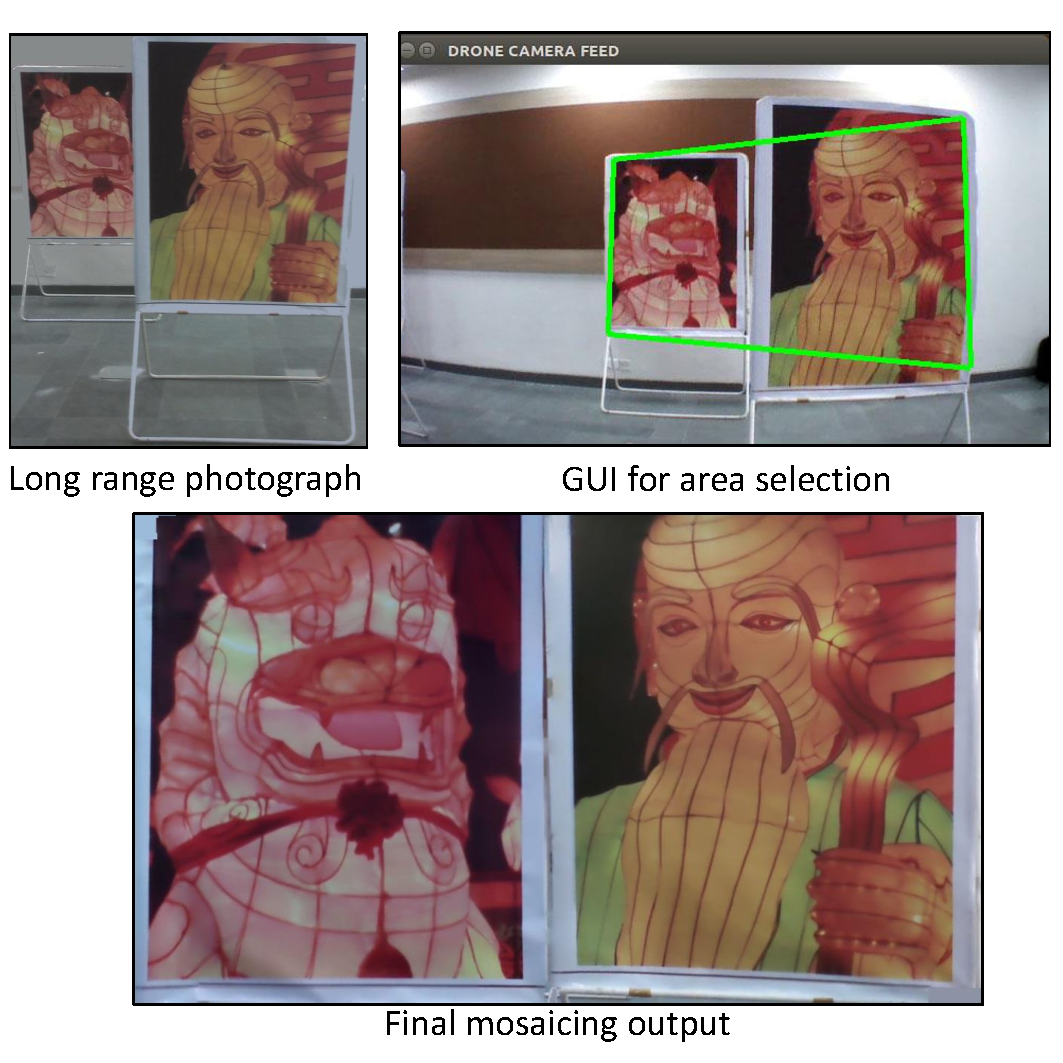
\includegraphics[width=\linewidth]{figures/multiplanar/frontback.pdf}
\caption[Result: Imaging at different depths]{There are two Chinese lanterns'
exhibits arranged parallel to each other but having different depths as shown in the long range
photograph(top-left). It is not able to mosaic both of them in a single
panorama due to the difference in depths. But we imaged those exhibits
independently through a quadcopter and brought the mosaic of an exhibit at larger
depth to the same depth of lesser depth exhibit mosaic. The final result is
shown in the bottom image.}
\label{fig:resultFrontBack}
\end{figure}

\section{Concluding remarks}
We have developed an end-to-end application for autonomously imaging multiplanar
regions using a quadcopter. We have also developed an algorithm for `unrolling'
the multiplanar scene using the fusion of IMU data and video captured from
quadcopter. Homography-based stitching cannot be used to create the mosaic of
scene spread over multiple planes. Also, using the handheld camera is cumbersome
to cover large multiplanar surfaces. Even with the UAVs manual control is very difficult.

In our solution, we autonomously maneuver quadcopter along the planned path to
cover each plane in a multiplanar surface. The path planning for each plane is
done to estimate optimal locations such that images from estimated locations will cover
the whole plane. Later, we stitch images for each plane to create mini-panorama.
Finally, mini-panoramas are merged using positional information to form a full panorama.
Our method works in various setups like convex, concave as well as mixed.

%In the future, our method may be extended to cover any parametric surface in
%general.
It is practically impossible to image very large multiplanar surface using
just single quadcopter due to battery constraint. We can use multiple
quadcopters in collaboration to overcome this limitation. However, we need to
identify each quadcopter accurately to send proper commands. Identification of
a moving object in the unknown environment is a challenging task. Generally, 
fiducial markers are placed on an object for tracking. Motion blur introduced
due to swift movements of quadcopter causes problem in detection of current
fiducials. We discuss the design of motion blur resilient fiducials as well as
the detection of the same in next chapter.
